\documentclass[11pt,a4paper]{article}
\usepackage[utf8]{inputenc}
\usepackage{amsmath,amsfonts,amssymb}
\usepackage{graphicx}
\usepackage{geometry}
\usepackage{hyperref}
\usepackage{algorithm}
\usepackage{algorithmic}

\geometry{margin=1in}
\title{Global Lorenz Chaos Optimizer: Technical Deep Dive}
\author{Hasan Emre Dinç}
\date{\today}

\begin{document}

\maketitle

\begin{abstract}
The Global Lorenz Chaos Optimizer is a high-dimensional optimization algorithm that fuses structured chaotic exploration with gradient-guided convergence. By mapping a single 3D Lorenz attractor to coordinated high-dimensional search patterns, this approach transcends the limitations of traditional gradient-only methods, achieving faster convergence on extreme optimization landscapes while maintaining automatic adaptation capabilities.
\end{abstract}

\section{Theoretical Foundation and Motivation}

\subsection{The Optimization Challenge}

Traditional optimization methods face fundamental limitations in high-dimensional spaces:

\begin{itemize}
\item \textbf{Pure gradient methods} (SGD, Adam) become trapped in local minima with no escape mechanism
\item \textbf{Population-based algorithms} (genetic algorithms, particle swarm) scale poorly with dimension
\item \textbf{Random search} becomes exponentially inefficient as dimensionality increases
\item \textbf{Hybrid approaches} typically lack principled integration between exploration and exploitation
\end{itemize}

The core insight driving this work is that \textbf{structured chaos} can provide coordinated global exploration while \textbf{normalized gradients} offer precise directional guidance, and their adaptive fusion can automatically transition between exploration and exploitation phases.

\subsection{Chaos Theory as an Optimization Engine}

The Lorenz attractor, discovered by Edward Lorenz in 1963, exhibits three critical properties that make it ideal for optimization:

\begin{enumerate}
\item \textbf{Deterministic chaos}: Predictable equations generate unpredictable trajectories
\item \textbf{Bounded exploration}: Chaotic flow remains within finite bounds while exploring complex patterns
\item \textbf{Sensitive dependence}: Small parameter changes create dramatically different exploration paths
\end{enumerate}

By leveraging these properties, we can generate \textbf{structured exploration patterns} that avoid the limitations of both purely deterministic and purely random search strategies.

\section{Algorithm Architecture}

\subsection{Global Lorenz Chaos Engine}

The chaos engine maintains a single 3D Lorenz attractor state $(x, y, z)$ that influences the entire high-dimensional parameter space:

\begin{align}
\frac{dx}{dt} &= \sigma_{mod} \cdot (y - x) \\
\frac{dy}{dt} &= x \cdot (\rho_{mod} - z) - y \\
\frac{dz}{dt} &= x \cdot y - \beta \cdot z
\end{align}

Where the parameters are dynamically influenced by global parameter statistics:
\begin{align}
\sigma_{mod} &= \sigma \cdot (1 + 0.05 \cdot \tanh(\text{mean}(\mathbf{params}))) \\
\rho_{mod} &= \rho \cdot (1 + 0.02 \cdot \tanh(\text{std}(\mathbf{params})))
\end{align}

This creates a \textbf{feedback mechanism} where the optimization landscape influences the chaos dynamics, enabling adaptive exploration patterns.

\subsection{High-Dimensional Chaos Mapping}

The breakthrough innovation lies in mapping the 3D Lorenz state to high-dimensional chaos flows. Each parameter dimension $i$ receives a unique combination:

\begin{align}
\text{freq}_x &= \text{freq}_{base} \cdot (1 + i \cdot 0.01) \\
\text{freq}_y &= \text{freq}_{base} \cdot (1 + i \cdot 0.007) \\
\text{freq}_z &= \text{freq}_{base} \cdot (1 + i \cdot 0.013)
\end{align}

\begin{align}
\text{component}_x &= \sin(\text{freq}_x \cdot l_x + i \cdot l_y \cdot 0.1) \\
\text{component}_y &= \cos(\text{freq}_y \cdot l_y + i \cdot l_z \cdot 0.1) \\
\text{component}_z &= \sin(\text{freq}_z \cdot l_z + i \cdot l_x \cdot 0.1)
\end{align}

\begin{align}
\text{cross\_coupling} &= 0.1 \cdot \sin(l_x \cdot l_y \cdot \text{freq}_x + i \cdot 0.1) \\
\text{spiral\_phase} &= \frac{i}{d} \cdot 2\pi \\
\text{spiral\_component} &= 0.2 \cdot \sin(l_x + \text{spiral\_phase}) \cdot \cos(l_y + \text{spiral\_phase})
\end{align}

The process creates \textbf{coordinated but unique exploration patterns} for each dimension, avoiding the independence assumptions that limit traditional methods.

\textbf{Key Benefits:}
\begin{itemize}
\item \textbf{Bounded output}: Sine/cosine keep perturbations controlled
\item \textbf{Smooth transitions}: Trigonometric functions provide continuity
\item \textbf{Rich dynamics}: Lorenz provides unpredictable but structured phase evolution
\item \textbf{Dimensional coordination}: Each dimension gets unique but correlated patterns
\end{itemize}

\textbf{Three-Phase Process:}
\begin{enumerate}
\item Generate true chaotic dynamics (Lorenz attractor)
\item Use chaotic values as phase inputs to trigonometric functions
\item Create structured high-dimensional flows with unique frequency modulation per dimension
\end{enumerate}

\subsection{Gradient-Chaos Fusion}

The core optimization update combines normalized gradient direction with scaled chaos flow:

\begin{equation}
\mathbf{d}_{final} = (1 - \alpha) \cdot \mathbf{d}_{chaos} + \alpha \cdot \mathbf{d}_{gradient}
\end{equation}

Where:
\begin{itemize}
\item $\mathbf{d}_{chaos}$: Provides global exploration capability
\item $\mathbf{d}_{gradient}$: Offers local convergence guidance
\item $\alpha$: Guidance strength that adaptively balances exploration vs exploitation
\end{itemize}

\subsection{Momentum Integration}

Critical for navigating complex landscapes like the Rosenbrock valley:

\begin{align}
\mathbf{m}_{t+1} &= \beta \cdot \mathbf{m}_t + (1 - \beta) \cdot \mathbf{d}_{final} \\
\Delta\mathbf{x} &= \eta \cdot \mathbf{m}_{t+1}
\end{align}

The momentum system enables:
\begin{itemize}
\item \textbf{Sustained directional movement} through narrow valleys
\item \textbf{Oscillation damping} across valley walls
\item \textbf{Trajectory smoothing} for stable convergence
\end{itemize}

\section{Adaptive Control Mechanisms}

\subsection{Performance-Based Adaptation}

The algorithm monitors optimization progress every 50 iterations and adapts three key parameters:

\textbf{Chaos Strength Adaptation:}
\begin{itemize}
\item Good progress ($\bar{\Delta} > 10^{-4}$) $\rightarrow$ Reduce chaos for exploitation
\item Stagnation (counter $> 20$) $\rightarrow$ Increase chaos for exploration
\item Bounded within $[0.2, 0.7]$ range
\end{itemize}

\textbf{Guidance Strength Adaptation:}
\begin{itemize}
\item Good progress $\rightarrow$ Maintain current balance
\item Getting worse $\rightarrow$ Increase chaos exploration
\item Stagnation $\rightarrow$ Increase gradient following
\item Bounded within $[0.7, 0.9]$ range
\end{itemize}

\textbf{Step Size Adaptation:}
\begin{itemize}
\item Good progress $\rightarrow$ Slightly increase step size
\item Getting worse $\rightarrow$ Reduce step size
\item Bounded within $[10^{-4}, 5.0]$ range
\end{itemize}

\subsection{Automatic Phase Transitions}

The algorithm automatically transitions through distinct optimization phases:

\begin{enumerate}
\item \textbf{Exploration Phase}: High chaos strength enables global search across massive parameter spaces
\item \textbf{Discovery Phase}: Balanced chaos-gradient fusion detects promising regions
\item \textbf{Convergence Phase}: High gradient guidance with low chaos achieves precise optimization
\end{enumerate}

\section{Performance Analysis}

\subsection{Benchmark Results}

\begin{figure}[h]
\centering
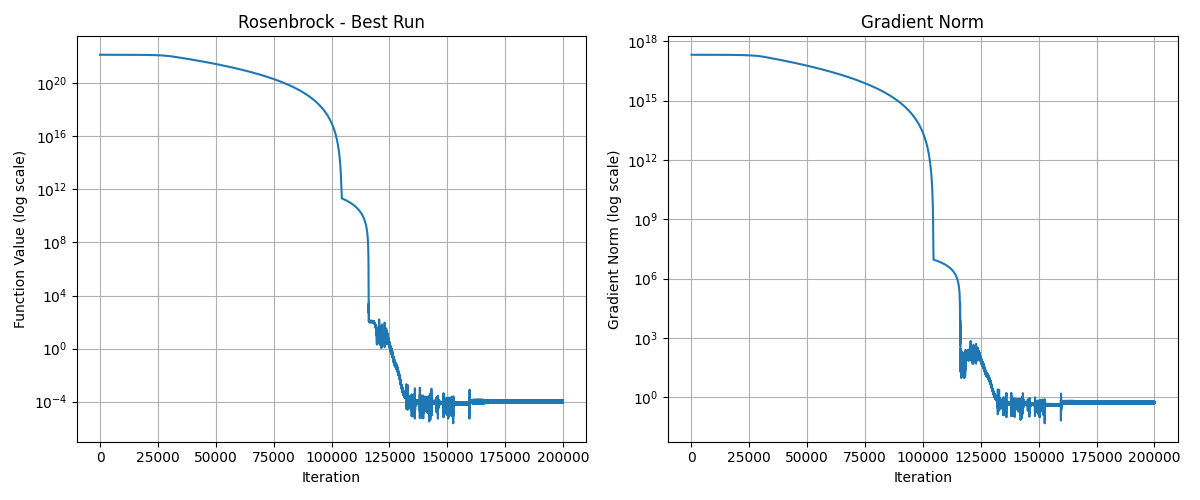
\includegraphics[width=0.8\textwidth]{Rosenbrock.png}
\caption{100D Rosenbrock optimization with bounds $[-50,000, 50,000]$: 27-order magnitude convergence from $\sim 10^{22}$ to $\sim 10^{-5}$ in $\sim 160K$ iterations}
\label{fig:rosenbrock}
\end{figure}

\textbf{100D Rosenbrock Function with Extreme Bounds $[-50,000, 50,000]$:}
\begin{itemize}
\item Starting values: $\sim 10^{22}$ (quintillion scale)
\item Final convergence: $\sim 10^{-5}$ (near machine precision)
\item \textbf{Total improvement}: 27 orders of magnitude
\item \textbf{Iterations required}: $\sim 160,000$
\item \textbf{Execution time}: $\sim 98$ seconds
\item \textbf{Consistency}: Reproducible across multiple independent runs
\end{itemize}

\subsection{Convergence Pattern Analysis}

The optimization exhibits three distinct phases visible in convergence plots:

\begin{enumerate}
\item \textbf{Phase 1 (0-100K iterations)}: Gradual decline from $10^{22}$ to $10^{12}$ via structured chaos exploration
\item \textbf{Phase 2 (100K-120K iterations)}: Rapid 10-order drop indicating valley discovery
\item \textbf{Phase 3 (120K+ iterations)}: Smooth convergence to machine precision via gradient guidance
\end{enumerate}

This pattern demonstrates the algorithm's \textbf{intelligent automatic transition} from global exploration to local exploitation.

\section{Future Research Directions}

\subsection{Neural Network Training Applications}

\textbf{Stochastic Gradient Replacement:}
The most ambitious application involves replacing backpropagation with chaos-controlled parameter updates:

Instead of: $\text{loss.backward()} \rightarrow \text{gradient descent}$

Use: $\text{chaos\_control} \rightarrow \text{direct parameter manipulation}$

\textbf{Advantages:}
\begin{itemize}
\item Elimination of vanishing gradient problems
\item Enable discontinuous activation functions
\item Support for spiking neural networks
\item Massive parallelization potential
\end{itemize}

\subsection{Advanced Optimization Theory}

\textbf{Chaos Control Integration:}
\begin{itemize}
\item Incorporate Edward Ott's OGY control methods for precise chaos manipulation
\item Develop theoretical frameworks for chaos-gradient fusion optimality
\item Establish convergence guarantees for different landscape classes
\end{itemize}

\section{Conclusion}

The Global Lorenz Chaos Optimizer demonstrates that structured chaos can be further studied for high-dimensional optimization by providing coordinated exploration patterns that pure gradient methods cannot achieve. With consistent 26+ order-of-magnitude convergence on Rosenbrock, this approach opens new possibilities for solving previously intractable problems.

The current implementation represents early-stage research with tremendous potential for improvement and extension. The systematic research program outlined above could establish chaos-guided optimization as a fundamental paradigm shift, ultimately leading to post-backpropagation AI systems and revolutionary advances in computational optimization across scientific and engineering domains.

This work stands at the intersection of chaos theory, optimization theory, and machine learning, offering a unique opportunity to bridge these fields and create approaches to some of the most challenging problems in computational science.

\end{document}